\chapter{Elliptic Curves} \label{AppA}
This appendix contains geometrical explanations and proofs for the group law on elliptic curves.
\\
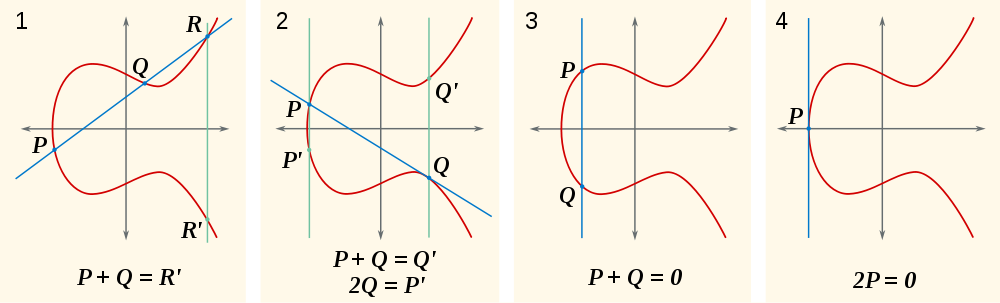
\includegraphics[width=\textwidth]{EllCurves}
\\
\\
The leftmost picture, labeled with $1$ shows that $P+Q=Q+P$, for it is easy to see that the line through $P$ and $Q$ remains the same.

The second picture ($2$) shows an expansion on the addition, wherein $Q+Q$ is calculated by taking the tangent to $Q$, arriving at $P$ which results in $Q+Q=P'$.

The third picture ($3$) shows both the existence of an inverse element, and the existence of a neutral element. Consider that any vertical line ends in the point $O$, the point at infinity. It is easy to see that the line through $O$ and $P$ ends up having a third point of intersection in $Q$, and that therefore $P+O=P$. Since it's already been shown that $P+O=P=O+P$ and therefore $O$ is the neutral element. Furthermore it is easy to see that $Q$ is the inverse element of $P$, since $P+Q=O$. Therefore it may be stated that $Q=-P$ and the existence of the inverse element has been proven.

The fourth picture ($4$) shows an interesting case, where the point on the curve at $x=0$ results in a point that is its own inverse, since $2P=O$ and $P-P=O$ so therefore in this case $P=-P$.
\\
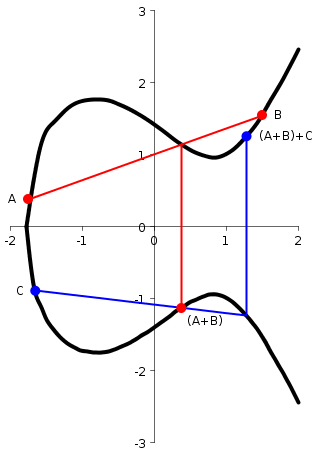
\includegraphics[width=0.5\textwidth]{EllAss1}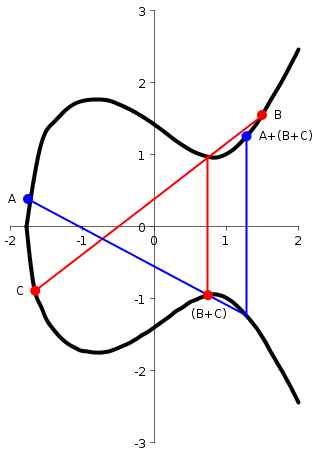
\includegraphics[width=0.5\textwidth]{EllAss2}
\\
\\
Finally associativity is shown by the two figures above. The left picture shows $(A+B)+C$, and the right picture shows $A+(B+C)$. It is easy to see that the points $A,B,C$ remained the same, and that, indeed, $(A+B)+C=A+(B+C)$.